%%%a general introduction into libpnicore


%%%============================================================================
\section{The PNI library stack}

%%%----------------------------------------------------------------------------
\begin{figure}[tb]
\centering
\resizebox{0.8\linewidth}{!}{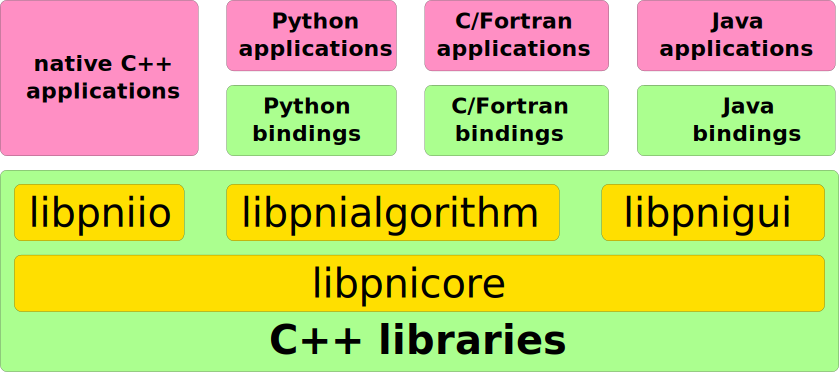
\includegraphics{pics/pni-cpp-libraries.pdf}}
\caption{{\small\label{fig:intro:libstack} 
The PNI library stack is a collection of C++ libraries developed with the
intention to simplify the process of writing application in the PNI field.
\libpnicore , the library described in this manual is the foundation of this
stack. It provides all the basic data structures and facilities used by all
other libraries.}}
\end{figure}
%%%----------------------------------------------------------------------------

\libpnicore\ is one of the PNI libraries developed within the framework of the
HDRI project. As shown in Fig.~\ref{fig:intro:libstack} \libpnicore\ it is the
foundation for all libraries in the stack. None of them can be used
without it. 
\libpnicore\ provides the basic data structures used by all other PNI libraries. 
This includes
\begin{itemize}
    \item well defined data types
    \item multidimensional arrays
    \item configuration facilities 
    \item type erasures.
\end{itemize}



%%%============================================================================
\section{How to read this manual}

For a new user the best way to read this manual is from beginning to the end.
One may can omit the next chapter about installation of the library if this is
done by your local system administrator. In any case, a new user should should
definitely start with Chapter~\ref{chapter:using_library}.

The library makes heavy use of C++11 features. There are plenty of websites on
the internet explaining those new features. For an experienced C++ programmer 
the Wiki site\cite{web:cpp11wiki} describing the new features for C++11 might be
enough. However, new users with less experience in modern C++ may should
purchase one of the excellent books available on this language.

A reader already familiar with \libpnicore\ may uses this guide as a short
reference to the most important features. In any case, more detailed information
about each class can be found in the API documentation.



